

\chapter{A longitudinal study of 15 million people to measure disease dynamics}
\label{longitude}

\section{Introduction}

%We now have a set of diagnoses, timestamps, and user locations for the period of the study. That is, we have the basis for a large-scale, high resolution disease surveillance system. Aside from the traditional problem of disease detection (see section \ref{www2014}), we can also use this high-resolution spatial data to parameterize models for the spread of the disease. 


An accurate model of disease transmission is necessary for efficient methods of disease control.\cite{yang2015inference,bilge2014uniqueness,newman2003social,salathe2010high,Smieszek:2013gg,world2006communicable,fraser2004factors,read2013determining,mossong2008social} However, disease transmission is often either estimated at a large scale, through population trends,\cite{yang2015inference,bilge2014uniqueness,diekmann2012mathematical,heesterbeek2002brief} or in small subsamples of estimated peer to peer transmission.\cite{salathe2010high,Smieszek:2013gg,klontz1989outbreak,moser1979outbreak,Cattuto:2010id,liem2005lack} Both of these approaches have flaws, however. Large scale, population trends require the development of costly disease surveillance systems\cite{yang2015inference,world2006communicable} and are only studied on a regional level. Additionally, these systems, which are often built on top of regional health providers, assumes that their samples are representative of the population as a whole. This may not be the case for relatively mild diseases, such as influenza, where only a small amount of the population may actually visit their doctor for treatment. For example, the CDC only recommends people in high risk groups to visit a health provider.\cite{cdcnoflu}  Small, peer-to-peer studies are also flawed due to issues related to determining who has actually come in contact with an infectious individual, the effort required to perform a study and the tendency for these studies to be retroactive.\cite{mossong2008social,salathe2010high,Smieszek:2013gg} 

Here, we develop a novel method of influenza transmission detection through a longitudinal analysis of 15 million Twitter users over a four year period. This approach addresses five of these six issues. Our approach can exploit data collected through third party social media platforms (in this chapter, Twitter) which is readily accessible instead of needing to partner with, or develop, a disease surveillance system. We use information provided by each user's GPS equipment to gain hyper-local information about the disease, compared to city, state or national regions provided by traditional surveillance systems. Twitter access is essentially free, compared to going to a health care provider which potentially reduces biases caused by socio-economic factors, although the Twitter population sample will introduce its own biases. We do not address the issue of determining actual contacts, although our results appear stable over a range of potential contact distances. As our system is automated, it scales well compared to traditional disease spread surveys. Finally, our data is collected in real time, eliminating issues related to subjects having a faulty recollection of past events.

In this chapter, we focus on the base reproductive number \(R_0\). Traditionally, research has calculated either \(R_0\) which is defined as the number of individuals a sick individual will infect over her disease's time span with the assumption that all other individuals are susceptible to infection or the effective reproductive rate \(R_E\).\cite{bilge2014uniqueness} The effective reproductive rate is easier to observe ``in the wild'' as it controls for the effects of unobserved resistance to disease or non-uniform mixing of the population.\cite{diekmann2012mathematical,heesterbeek2002brief} Hence, we can track each individual in our subpopulation to estimate the amount of resistance and network effects, allowing us to calculate the base reproductive number to be 2.6945.

The remainder of this chapter is organized as follows. In section \ref{sec:diagnosissystem}, describe the modifications to the classifier built in chapter \ref{www2014} to scale to our larger dataset. In section \ref{subsec:datacollection} we describe the collection, storage and processing of our large Tweet dataset. In section \ref{sec:curvefitting}, we describe a classical method of determining \(R_0\) and our system can replicate this method. In section \ref{methods:individual}, we develop a novel form of disease modeling to determine \(R_0\) that employees additional data our Twitter-based-surveillance-system provides. In section \ref{sec:resultsLongitude}, we compare the results of our methods to previous studies' results.  Finally, we conclude by describing potential biases--due to our inferred contact networks (section \ref{discussion:contacts}) and spam messages (section \ref{sec:spam})--along with our approaches to controlling for them.


\section{Methods}
\subsection{Building a Validated Diagnosis System}
\label{sec:diagnosissystem}
We begin by developing a system that is capable of accurately assessing influenza cases in individuals based on their Twitter feeds. To do this, we collected data on 104 Twitter users that were \emph{professionally} diagnosed with influenza, and 122 Twitter users that self reported as \emph{not} having any influenza-like-illnesses during a one year period of data collection as described above, in chapter \ref{www2014}.  Next we trained a machine-learning classifier to differentiate between these two user groups. To allow the classifier to scale, we do not include the long term tweeting rates, followers network, or hand rated Tweets into this version of the classifier. The simplified version of the classifier performed with an accuracy of \(89.72\%\) and an area under the ROC curve of \(0.8544\). (See the previous chapter for further details.) Since an influenza infection is acute, we grouped each user's time line into monthly slices, which is defined as being a time of illness if the user was professionally diagnosed during that non-overlapping window. 

We then apply the classifier to each user's time-line on the 4-week sliding window, with each step of the sliding window being one day. The classifier assigns a score to the day where the sliding window begins based on the Tweets the user has posted within the window. For example, when the sliding window first encounters a user's Tweet that says ``I am getting sick with the flu,'' the classifier will heavily lean toward her being sick. Later, the user may Tweet ``I am no longer sick'' which will give a strong signal that the user is no longer sick which will tend to outweigh the user's previous ``sick'' Tweet even if they both occur in the same window. Of course, it is rare that such strong signals are in the data, so the classifier is built on an amalgamation of many weaker signals---mentioning going to a party as a not-sick signal, for example---which, while weaker, are more prevalent. We chose a step size of one day in order to increase the temporal granularity of the classifier. Users that are inactive for more than 30 days are not included for \emph{any} analysis during that time window.

%When this score is above a cutoff--determined during the classifier's training--the user is classified as ``sick'', otherwise she is classified as ``not sick'' on that day. 


\subsection{Twitter Data Collection}
\label{subsec:datacollection}
We collected almost all Tweets from the continental United States with high-resolution geo-spatial information over a four year period from March \(3^{rd}\) 2011 to March \(4^{th}\) 2015. Twitter allows users with GPS equipped devices such as mobile phones to opt in to sharing high-resolution geospatial data with each of their Tweets. This data is mainly (\(> 99\%\) of the time) as a point defined by longitude and latitude, with the remaining portion consisting of bounding boxes. For compatibility, we converted these bounding boxes to the midpoint of the box. To collect this data we queried Twitter's streaming API with a request for a bounding box that covers the area in interest, thus insuring the collection of geo-taged Tweets with high resolution geo-spatial information. While this limits our data collection to a subset of all Twitter users, it has two substantial advantages. First, the high geospatial resolution allows us to study patterns that occur over short distances, such as disease transmission. Second, this geo-filter allows us to obtain almost all Tweets that match our filtering criteria without invoking Twitter's rate limits.\cite{morstatter2013sample} A total of 2,732,174,105 Tweets from 15,560,328 users were collected during this four year time period.

The collected Tweets were then processed through a combination of custom Hadoop programs and Apache Hive scripts on Amazon's Web Services. Each Tweet, when collected through the Twitter API, is associated with a variety of metadata. We parsed each Tweet and stored a simplified version containing user id, the Tweet's text, the time the Tweet was posted and the latitude and longitude describing the location where the Tweet was posted and stored it on a Hadoop Distributed File System. Each user--identified by user id--is then tested for disease based on the method described above in section \ref{sec:diagnosissystem} for each day that he or she was active. We discard users from our dataset who Tweeted less than 10 times over the entire four year period, as it is unlikely that they will have provided enough data to be useful. Finally, we determine the location of each user based on her longitude and latitude and store her state and HHS (Health and Human Services) region. This was then done by finding the mean location of each user by averaging all of the locations of her Tweets. Then, the user's location is then mapped to a state (or District of Columbia) using a hive plug-in \footnote{https://github.com/ToddBodnar/GeoUDF}. Users that were \emph{not} in any state tended to be in northern Mexico or southern Canada and were discarded from analysis. Each HHS region is simply an aggregation of several states, making it relatively easy to convert from state to region. 

\subsection{Estimating Transmission Parameters}

\subsubsection{Parameter estimation through curve fitting}
\label{sec:curvefitting}

While the above system has been shown to perform well on the case study data\cite{Bodnar:2014:GVO:2567948.2579272}, the data may be biased, limiting the classifier's ability to generalize to an arbitrary set of Twitter users. To show that this isn't the case, we consider applying our classifier to our full, high-resolution geospatial Twitter dataset. If trends discerned from this application match previously measured real-world results from the CDC, then we will gain some confidence on our system's ability to generalize. Here, we consider the traditional approach of determining the basic reproduction number, \(R_0\), at the population level. To do this, we consider a SIR (Susceptible-Infectious-Recovered) model of disease. First, we build these models using the standard transition equations for the SIR model:


\begin{equation}
\frac{dS}{dt} = -SI\beta ,\;\; \;\; \;\; \;\;  \frac{dI}{dt} = SI\beta - I\gamma, \;\;\;\; \;\; \;\;  \frac{dR}{rt} = I\gamma
\end{equation}


Where \(S\),\(I\) and \(R\) are the frequencies of susceptible, exposed, infectious and recovered individuals, respectively.\cite{heesterbeek2002brief} Note that the parameters \(\beta\) and \(\gamma\) are the transition probabilities from being susceptible to having the disease and recovering from the disease, respectively. Additionally, we could consider SEIR models for parameter fitting. However, recent work has shown that inferences made from SIR models out perform inferences made by more complex models such as SEIR \cite{diekmann2012mathematical,yang2015inference} and that solutions for SEIR models are not unique \cite{bilge2014uniqueness}. Additionally, ``[a] single-age class SIRS model inference system is able to reliably infer the leading eigenvalue of the effective reproductive number.'' \cite{yang2015inference} As the purpose of this section is to just give a base-line for user-based analysis, we do not further consider SEIR models as SIR models are simpler and more accurate.

We can now find the parameters of \(\beta\), \(\gamma\) and starting values for \(S\), \(I\) and \(R\) that cause the model to best fit our data using a multi-grid search. Specifically, we search through three variables, the two transmission parameters \(\gamma\) and \(\beta\) and \(S(0)\), the initial susceptibility rate which may be less than 1 due to innate immunity or previous vaccination. 
%: \(3^{-11} \leq \gamma \leq 3^9\) and \(3^{-11} \leq \beta \leq 7.5 \times 3^9\). Note that these ranges are significantly wider than reasonable parameter values as we do not want to preclude any reasonable values. 
Next, we generate a logarithmically spaced 25 by 25 by 25 grid of potential values over this range. We then set \(I(0)\) to be the same as the first infection value in the data and \(R(0)\). We then solve an SIR model, with each of the parameter combinations. Finally, we compare the results of the model to the data based on 
\begin{equation}
error = \sum_t (I_{\gamma,\beta}(t) - I_{data}(t))^2
\end{equation}
 We then find the value of \(\gamma\) and \(\beta\) which have the smallest error. We then recenter the variable's ranges on these new values and reduce the range to search by an order of magnitude. This process is repeated 25 times, at which point the minimum and maximum range tested differed less than the machine's precision (\(\approx 2\times 10^{-16}\)).

%% (i.e. \(\gamma_i = 3^{20/24 * i - 11}\), \(i = 0,2, ... 24\) for the initially tested values of \(\gamma\))

We can generalize this method to either arbitrary subset of any (from the CDC or generated from Twitter) disease incidence curve by comparing the SIR model for a given \(\gamma,\beta\) pair to just a subset of the time-steps or to multiple incidence curves. Note that one could employ more efficient methods of parameter fitting such as Euler's method,\cite{diekmann2012mathematical} likelihood estimation\cite{yang2015inference} or genetic algorithms,\cite{banzhaf1998genetic} however, the small number of parameters and the reasonably small number of time steps in each incidence curves allow for a naive grid-search to be executed quickly.


Because the influenza virus constantly mutates between flu seasons, previous infection does not necessarily confer a resistance to future infections. For example Cowling et al. \cite{cowling2010protective} do not find a significant difference in seasonal influenza rates based on the previous year's vaccination. To simplify our analysis, we model each year separately, not assuming any cross-protection. We consider both sharing the same values of parameters for every year and refitting the model to each year. As we have geographical information, we additionally build these models for each of the 10 HHS (U.S. Health and Human Services) regions. As a proof of concept, we also perform these methods on the county level. Specifically we use Tarrant County in the state Texas and King county in the state of Washington as two case studies. These locations were chosen due the public availably of surveillance data from the local public health institutions. Note that both of these counties have large population sizes, with Seattle, Washington and Fort Worth, Texas being two large cities in those two counties, respectively. From each of these models, we calculate \(R_0\) based on the estimated parameters by using the relationship

\begin{equation}
\label{eq:r0}
R_0 = \frac{\beta}{\gamma}.
\end{equation}

\subsubsection{Parameter estimation through individual user analysis}
\label{methods:individual}
Next, we consider employing both the high-resolution spatial data and the individual Twitter-based diagnoses to develop a network-based model of disease transmission. We begin by constructing a pseudo-contact network between each of the Twitter users based on their geo-spatial information in our dataset. We consider two users to be in contact if they are less than a distance \(d\) from each other. We assign the health state (sick or not sick) to each user to the network at a daily temporal resolution. From this, we can determine whether or not being located near a sick user increases one's likelihood of getting sick shortly after the potential exposure. While the Twitter users in our dataset are only a small subsample of the general population, we would still expect to see this effect in our data due to the close (droplet-borne or airborne) proximity requirement of influenza transmission. \cite{weinstein2003transmission,liem2005lack,cowling2009facemasks}

Additionally, we estimate \(R_0\) for the disease from the individual infections as follows. As with the disease transmission likelihood estimation above, we begin by considering neighboring users that were ill previous to the time that an user became ill as potential candidates as being the exposing individual. Since we cannot determine which of the \(i\) ill neighbors infected the individual, we assign each ill neighbor \(\frac{1}{i}^{th}\) of the responsibility for infecting the individual. Each user's cumulative responsibility for infecting \emph{all} other cases of illness is then the expected number of people the user has infected. We then calculate the average \(R_0\) of the disease by averaging the expected number of infections for all of the users that were sick.

When determining the responsibility of infection, we assume that an individual became infected the first day that she is classified as being ill, minus a lag \(l_t\), that we vary in the model. This lag is due to both the incubation period and the fact that individuals do not necessarily report symptoms to Twitter on their first day of illness. Additionally, we assume that an individual gains an immunity to the specific strain of influenza after becoming ill and will thus not become infected again until the next flu season.



\section{Results}
\label{sec:resultsLongitude}

\begin{figure}
\centering
\begin{subfigure}[b]{0.3\textwidth}
	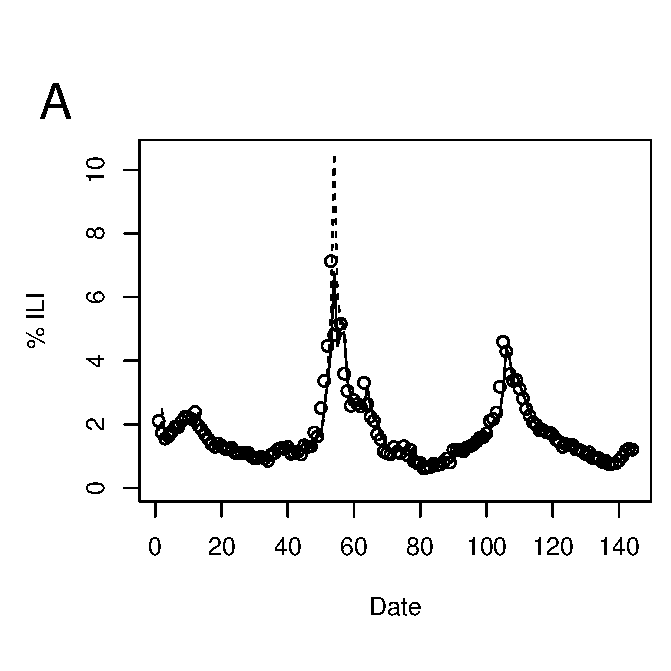
\includegraphics[width=\textwidth]{longitude/figs/nowcastNational.eps}
\end{subfigure}
\begin{subfigure}[b]{0.3\textwidth}
	\includegraphics[width=\textwidth]{longitude/figs/nowcastHHSExample.eps}
\end{subfigure}
\begin{subfigure}[b]{0.3\textwidth}
	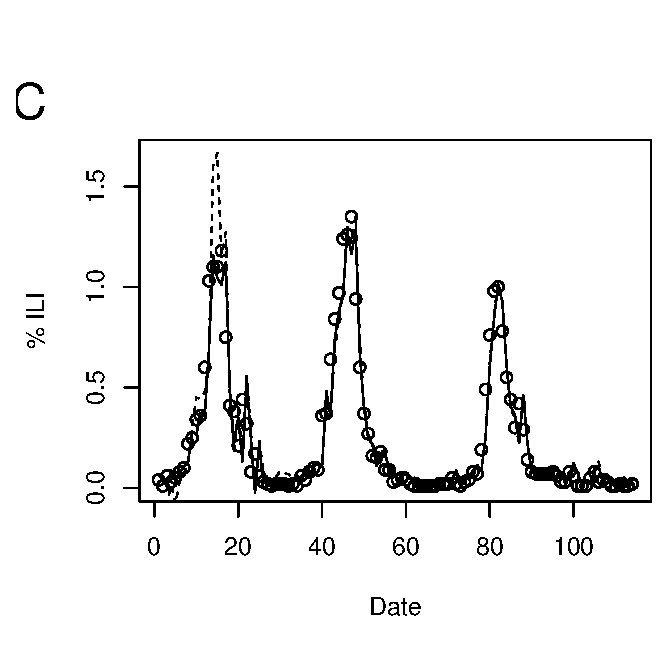
\includegraphics[width=\textwidth]{longitude/figs/nowcastLocalExample.eps}
\end{subfigure}
\caption{Comparison of Twitter's forecasting (dashed lines) and retroactive measurements (solid lines) to the CDC's reported Influenza rates (circles) for national (A), HHS Region 1 (B), and Seattle area (C).}
\label{fig:curves}
\end{figure}



\begin{table}[h]
\centering
\begin{tabular}{lcc}
Flu Season & CDC Data & Twitter Data\\   \midrule
 \rowcolor{lightblue} 2011-2012&  2.053 &  1.997\\ 

2012-2013& 2.044 &  2.200\\ 

\rowcolor{lightblue} 2013-2014& 2.044&  2.178 \\ 

Combined& 1.854  &  2.087 \\
\end{tabular}
\captionsetup{singlelinecheck=off}
\caption[Estimated R0 based on CDC and Twitter data]{Estimated \(R_0\) based on CDC and Twitter data.}
%%run full_region_year.r
\label{tab:nationalr0}
\end{table}



%\begin{landscape}
\begin{table}[h]
\begin{tabular}{ccccc}

 Year & \(\gamma\) & \(\beta\) & Sum Square Error\\ \hline
& 0.1732 & 0.1749  & 0.0001047   \\ 
 {\multirow{-2}{*}{ 2011-2012 }}  & \cellcolor{lightblue} 0.1176  & \cellcolor{lightblue} 0.1195  & \cellcolor{lightblue} 0.0001323  \\ \cline{2-4}
  {\multirow{2}{*}{ 2012-2013 }}& 0.7715 & 0.9626 & 0.0009402   \\ 
   & \cellcolor{lightblue} 0.7317  & \cellcolor{lightblue} 0.9020 & \cellcolor{lightblue} 0.0009492   \\ \cline{2-4}
  {\multirow{2}{*}{ 2013-2014 }}& 0.6054 & 0.7288   & 0.0003114   \\ 
   & \cellcolor{lightblue} 0.6046 & \cellcolor{lightblue} 0.7264 & \cellcolor{lightblue} 0.0003026  \\ \cline{2-4}
  {\multirow{2}{*}{ Combined }}& 0.6998 & 0.8225  & 0.003719   \\ 
   & \cellcolor{lightblue} 0.6765  & \cellcolor{lightblue} 0.7935  & \cellcolor{lightblue} 0.003252   \\ 
\end{tabular}
\caption{National best-fit parameters for each year from the CDC's data (white) and Twitter data (gray).}
\label{tab:nationalparams}
\end{table}
%\end{landscape} %%SSE percentiles removed for space

\begin{table}[h]
\centering
\begin{tabular}{cccc}
County & Flu Season & CDC Estimates & Twitter Estimates  \\ \hline& 2011-2012 & 1.14  &  1.14   \\ 
\rowcolor{lightblue} \cellcolor{white} & 2012-2013  & 1.542  &  1.576  \\ 
  &  2013-2014 & 1.454&  1.443 \\ 
\rowcolor{lightblue} \cellcolor{white} 
 {\multirow{-4}{*}{ Fort Worth }}  &  Combined  & 1.375&  1.38\\ \hline
 & 2011-2012 & 6.073  &  4.934 \\ 
\rowcolor{lightblue} \cellcolor{white}   & 2012-2013  & 11.7&  11.7 \\ 
  &  2013-2014 & 1.000 &  1.117  \\
\rowcolor{lightblue} \cellcolor{white}  {\multirow{-4}{*}{ Seattle }}& Combined  & 4.053 &  3.415 \\
\end{tabular}

\captionsetup{singlelinecheck=off}
\caption[Estimated transmission based on CDC and Twitter data.]{Estimated \(R_0\)  based on CDC and Twitter data with 5\% and 95\% percentiles in parentheses for the two proof-of-concept county datasets. Additionally, T-Tests and Kolmogorov-Smirnov Tests are performed to compare results.}
\label{tab:localr0}
%%
\end{table}


\begin{figure}
\centering
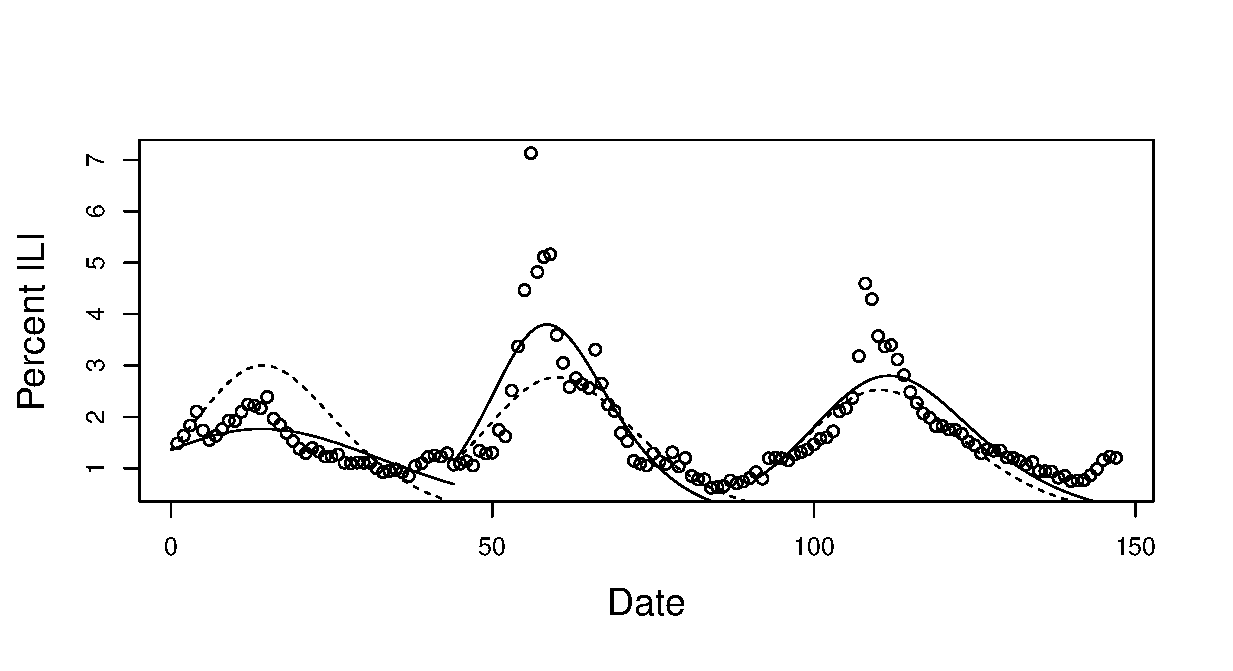
\includegraphics[width=1.0\textwidth]{longitude/figs/sirCurve.eps}
\caption{The CDC's estimates (circles) of influenza rates for a three year period compared to the best fit SIR models from the Twitter data using combined (dashed line) or yearly (solid line) parameters.}
\label{fig:sirFit}
\end{figure}

\subsection{User Activity Summaries}

Before discarding low-activity users, our dataset consisted of 2,732,174,105 Tweets from 15,560,328 users, resulting in a mean of 175.59 Tweets posted per user. The tweet count distribution was highly dispersed, with a maximum of 1,119,384 Tweets  (approximately 767 Tweets per day), a median of 10 Tweets, and a minimum of one Tweet over the study period. On the lower end of the spectrum, it is unlikely that users who posted less than 10 Tweets over the 4 year period will have provided us much information. Therefore, as described above, we discarded them from our dataset for our analyses. On the other hand of the spectrum, the group of most prolific Twitter users may contain automated spam bots. As we describe in section \ref{sec:spam}, we used Twitter's API to identify spam bots and found 3\% of the users to be spam-bots, but removing them did not significantly effect our main results. 

%%Total Tweet rates over time, just show increase of Tweeting rates. May be unnecessary.

The geo-spatial distribution of the Twitter users appears consistent with the U.S. population distribution. To validate this observation, we determined in which county the user is located by comparing, for each user, the mean longitude and latitude of their Tweets to the US Census Bureau's county shape files.\footnote{https://www.census.gov/geo/maps-data/data/tiger-line.html} We then compared the count of users in each county with the 2010 Census population count and find a strong relationship (Spearman's \(\rho = 0.708\), see figure \ref{fig:census}). As both the Twitter user count and Census population count follow a long tail distribution, they are first log-transformed before compared by Pearson's coorelation coefficient. 

\begin{figure}
\centering
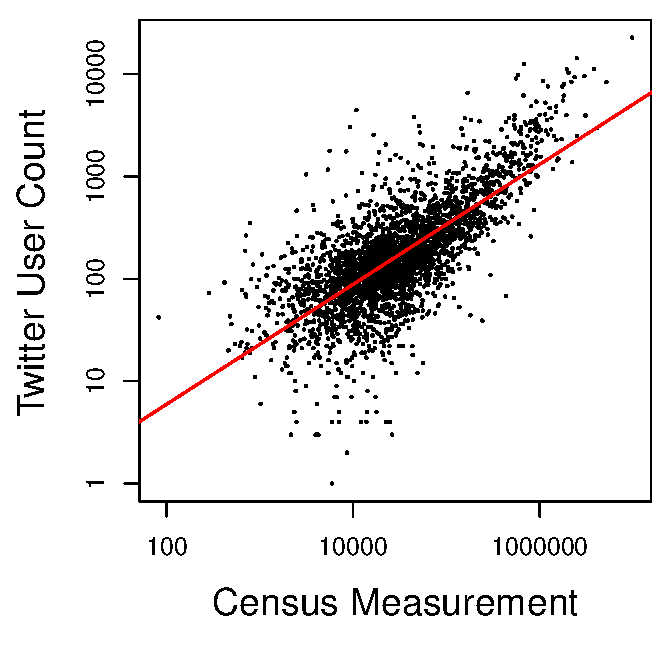
\includegraphics[width=.5\textwidth]{longitude/figs/compare_twitter_census.eps}
\caption{The relationship between the US Census's population count and number of Twitter users in our dataset.}
\label{fig:census}
\end{figure}

\begin{table}[h]
\centering
\begin{tabular}{cccc}
Distance (km) & \(\bar{K}\) & Variance(K) & \(1+Variance(K)/(\bar{K}^2-\bar{K})\) \\ \midrule
~~0.1      ~~    &     42110.48     &    \(  4.1911\times10^{10}\)     &     3.3635     \\ 
\rowcolor{lightblue}  ~~0.5      ~~   &      42144.56     &     \(4.1973  \times10^{10}\)     &     3.3632 \\ 
~~ 1.0   ~~       &      42155.25     &     \( 4.1989  \times10^{10}\)    &     3.3629     \\
\rowcolor{lightblue} ~~ 5.0   ~~      &      42383.88     &      \( 4.2267 \times10^{10}\)    &       3.3529    \\ 
~ 10.0      ~~    &       43089.55    &     \( 4.3101\times10^{10}\)      &    3.3214       \\ 
\rowcolor{lightblue} ~ 50.0   ~~      &       63776.20    &      \(6.9418  \times10^{10}\)    &        2.7067   \\ 
100.0  ~~        &       112829.72    &      \( 1.6611  \times10^{11}\)   &      2.3049     \\ 
\end{tabular}
\captionsetup{singlelinecheck=off}
\caption[The average and variance of the number of other users that are within a given user of a distance and the R0 modification factor.]{The average and variance of the number of other users that are within a given user of a distance and the \(R_0\) modification factor.}
\label{tab:ro_adjustment}
%%generate by running hiveInfectionSummary.approxK.main and then execute
%% CREATE TABLE neighbors(distance FLOAT,count INT) ROW FORMAT DELIMITED FIELDS TERMINATED BY ',';LOAD DATA INPATH './neighbors/' INTO TABLE neighbors;select distance, AVG(count), VAR_pop(count), 1 + VAR_pop(count)/(AVG(count)*AVG(count)-AVG(count)) from neighbors group by distance order by distance;
\end{table}

\subsection{Diagnostic Validation}
\label{subsec:validation}
Before we use our Twitter diagnoses as a proxy for actual disease measurements to determine disease transmission parameters, we must first validate that our diagnoses match expected trends. We have previously shown that our diagnoses classify professional diagnoses of a small sample of Twitter users relatively well, but it is possible that the small sample size of that study biases our diagnostic method in a way that limits its ability to generalize to the full population of Twitter users. To investigate this possible bias, we aggregated all of our users in an area, use our classifier to assess disease status and then calculate the disease incidence based on our classification. If there were a strong bias to our classifier, these Twitter incidence curves would \emph{not} be expected to match with the CDC's incidences curves.

Here, we present the comparison of those incidence curves, i.e. from our Twitter data and the CDC data. The incidence of disease is not normally distributed, hence we use Spearman's rank correlation coefficient instead of Pearson's correlation.  We note that our measurements perform well, with the fit at the national scale (\(\rho^2 = 0.90761\)) out performing Google Flu Trends (\(\rho ^2= 0.8207\)). We find that the regional ( \(0.8113 \leq \rho^2 \leq 0.9467\) in each HHS region) and local measurements for Tarrant county (\(\rho^2 = 0.8944\)) and for the Seattle area (\(\rho^2 = 0.7295\)) also fit well. Additionally, we look at the predictive power of the model by  training the model on data from weeks \(1...t-1\) and assessing its ability to predict the incidence at time \(t\). While these models are not as effective as models that fit to the entire dataset, they do perform well on the national \((\rho^2 = 0.90761)\), regional \( (\rho^2 = 0.9385)\), and local \( (\rho^2 = 0.6976)\) scale. For brevity, only one representative regional and local fit are presented in the main paper (see figure \ref{fig:curves}). Full model fits are available in appendix figures \ref{fig:hhs_curves_all} and \ref{fig:local_curves_all}.

 %While we do not intend to directly compete with advanced influenza now-casting methodology[], 

As described in section \ref{sec:curvefitting}, we estimate national-level influenza disease parameters,\(\beta\) and \(\gamma\),  based on the CDC and Twitter incidence curves. We find that the resulting estimate \(R_0\), based on the CDC data and our Twitter data do not differ substantially on the national scale (min difference = 0.002, max difference = 0.015, see table \ref{tab:nationalr0}) or for the regional scale data (min difference = \(2.725\times 10^{-4}\) , max difference = 0.106, mean difference = 0.0254, see table \ref{tab:hhsr0}), except for one region and one year (HHS Region 3, 2011-2012) where the Twitter estimate for \(R_0\) was 501\% higher than the \(R_0\) estimate from the CDC, possibly due to relatively small data size in the first year or the mild flu season. Additionally, the \(R_0\) for the two sample counties is estimated well by our Twitter data (min difference = \(2.754 \times 10^{-4}\)
, max difference = 1.139, mean difference = 0.2168, see table \ref{tab:localr0}), but not as closely as the regional or national datasets, possibly due to the small scale of county level data. Note that we also  estimated values of \(R_0\) based on the assumption that the transmission parameters do not vary between seasons, but the model does not fit the data as well (see figure \ref{fig:sirFit}) and thus is not included in the analysis.



\begin{figure}
\centering
\includegraphics[width=1.0\textwidth]{longitude/figs/r0_by_distance_time_new.png}
\caption{Estimated peer-to-peer transmission rates based on maximum distances between users.}
\label{fig:r0distance}
\end{figure}

\subsection{Individual Parameter Fitting}




%While it is expected that population density has a long-tail distribution, we must control for this when calculating \(R_0\). 

The base derivation of \(R_0\), as in equation \ref{eq:r0}, assumes that each individual has the same number of contacts. However, it's been long know that this assumption is often invalid and that contact networks can exhibit substantial variation in the distribution of contacts. This increased variance, when not taken into account will lead to an underestimation of  \(R_0\) \cite{newman2003social,olinky2004unexpected,molina2012modelling} and is thus typically adjusted using the formula 

\begin{equation}
\hat{R_0} = R_0 \left(1 + \frac{variance(k)}{\bar{k}^2 - \bar{k}}\right)
\end{equation}
where \(\hat{R_0}\) is the adjusted version of \(R_0\) and \(k\) is the number of contacts.\cite{newman2003social,molina2012modelling} Note that in the case of a uniform distribution of contacts, the variance of \(k\) is zero and the adjusted version  \(\hat{R_0}\) is identical to \(R_0\). 

Here, we begin to calculate this adjustment by determining \(k_u(d)\), the number of neighbors of user \(u\) given a search distance of \(d\). This is done by iterating through all users and counting the number of additional users that are within \(d\) of each user. Note that since Twitter's geolocation is based on longitude and latitude, the distances must be converted into kilometers before compared. We can now calculate the mean and variance of \(k\) between each user for a given distance and  calculate the necessary adjustment to \(R_0\) (see table \ref{tab:ro_adjustment}).


We then apply this long tail adjustment to the mean cumulative infection responsibility calculated above (see table \ref{tab:ro_adjustment}) to determine the value of \(R_0\) for a given maximum distance and incubation period. Note that these effects are similar for a range of distances and lags (see figure \ref{fig:r0heatmap}). The incubation is not significantly different for values less than or equal to 12 days (p > .05 after adjustment, pair wise, logs scaled, t-test). As it would be unwieldy to report all combinations of these values, we choose to only report based on a lag of 7 days and a maximum distance of one km.



\begin{figure}
\centering
\includegraphics[width=0.75\textwidth]{longitude/figs/r0heatmap.png}
\caption[Effects of differing time and temporal windows on predicted R0. Note the increase in time after 14 days.]{Effects of differing time and temporal windows on predicted \(R_0\). Note the increase in time after 14 days.}
\label{fig:r0heatmap}
\end{figure}


With these parameters set, we can now study the flow of disease between users. We find a total of 182,801 infectious users. Note that we cannot detect all infections, as there are individuals that a user may have infected that were not in our dataset. We find that the adjusted number of expected infections an individual causes follows a long tail distribution (min = 0, max = 379.6000, mean = 2.6940, median = 0.8407, std = 6.8069, see figure \ref{fig:r0distribution}). 


\begin{figure}
\centering
\includegraphics[width=0.75\textwidth]{longitude/figs/r0distribution.png}
\caption{The adjusted number of individuals that a person is likely to infect during her disease. Note that the log-transformed x-axis does not include cases where zero transmission occurs.}
\label{fig:r0distribution}
\end{figure}




%See that r0 roughly .8. Mention ``super spreader'' dynamics, with an individual being assigned a total of \(\approx 60\) infections. Maybe mention targeting these people? 


%Then adjust for long-tail effects (using adjustments in table \ref{tab:ro_adjustment}) and find more reasonable numbers. (See figure \ref{fig:r0distance})




%Note that, when reported on a logarithmic x-axis (see figure \ref{fig:r0distance}), the effects of maximum-search distance on observed \(R_0\) appears to be logistic-like. Indeed, if we fit a modified, 4-parameter logistic equation
%\begin{equation}
%R_0(distance) = min_{R_0} + \frac{max_{R_0} - min_{R_0}}{1 + e^{-\alpha(log(distance) - \beta)}}
%\end{equation}
%where X is A and Y is B, we find a good fit (\(R^2 = XXX\)). We can then use this fitted model to estimate a 'global' \(R_0\) as measured through our agent-based method. Thus, when we allow \(distance \to \inf\), we find \(R_0(\inf)\) to be \( XX < 1.0\) in each of the four years indicating ---something about spatial dynamics---. Additionally, we can solve for Max Distance given the logistic curve and the population based \(R_0\) measurements. ---Not sure how to interpret, numbers will be around 20km. Possibly average movement??.

\section{Discussion and Future Work}

\subsection{Describing Pseudo-contacts}
\label{discussion:contacts}
Note that our definition of contact for disease transmission does not necessarily represent true contacts. Indeed, as we are only working with a subset of the entire population---people in the United States that are active Twitter users with geotagging activated---we can make no claims about \emph{all} contacts and transmissions being recorded. Hence, we likely incorrectly observe transmissions from user A to user B which actually involve a transmission from user A to user C to user B. This may also account for our model being consistent when the incubation period is set to two weeks, which is longer than the infection's length. \cite{thompson2004influenza}

Additionally, we are limited to the accuracy of the user's GPS when it comes to determining the distance between two users. Previous work by Glidden et al. \cite{yelpgps} find that, unlike previous claims\cite{zandbergen2011positional,djuknic2001geolocation,modsching2006field}, personal GPS devices do \emph{not} have sub-meter accuracy. For example, they find that more than 80\% of iPhone users are within 0.5 miles of where their GPS reports them to be and 4.5\% of iPhone users were more than 2 miles away from their reported location. Indeed, this appears that Twitter controls for this by limiting the reported locations. We find that 99\% of users with two tweets Tweet in the \emph{exact} location, with a mean of 8.79074e-5 degrees (\(\approx 9.8\) meters). This may also be an attempt by Twitter to limit user's from releasing private information about themselves (for example, see \cite{defcon}). %ref: defcon talk on walter reed doctor, rob-me website
While this limits our ability to accurately work on sub-kilometer distances, it also allows us to average each user's location across time to simplify the contact network to a static set of connections (although users/nodes vary over time due to user activity). 
%Pseudo-contact network is justifiable because while not actual contacts, we may also detect intermediaries (i.e. We survey users A and B, with A infection B, but in reality, A infects C who infects B) so we're still measuring the overall flow, just at a limited (but still much better than other paper's) resolution.

%Mean of locations are justifiable because small general range, min = 0, mean = 8.79074e-5, median = 95 percentile = 99 percentile = 0, 99.99 percentile = 0.0362 degrees (zero is probably due to gps accuracy of x meters?)

%\subsection{Going forward}
%Mentioning targeting super spreaders?

\subsection{Spam Removal}
\label{sec:spam}
So far, we have assumed that all of the collected Twitter accounts may provide accurate information about a person's disease state. However, this is not the case. Specifically, spam ``social'' bots \cite{boshmaf2011socialbot} may attempt to emulate real users, but their disease state would be meaningless. Indeed, much work\cite{Krause:2012uz,Biro:2008wd,Anonymous:iQRVCsVz} has been done on the topic of automated spam-account detection on Twitter. However, reproducing these papers' work appears difficult as they tend to rely on large, unaccessible hand coded data. Instead, we consider using Twitter's own API as a method to detect spam bots.

While Twitter does not directly supply a spam-API, attempting to look up a user that was banned results in a specific error returned, instead of the user's data. This method will overestimate the incidence of false accounts, as Twitter users can be banned for non-spam actions such as hate speech or copyright infringement. However, for our case this is acceptable since any effects from removing banned accounts will overestimate the effects from removing the subset of banned accounts that were bots. Additionally, while no spam detection system is perfect, it is likely that Twitter, itself, has a stronger motivation, more resources, and access to additional meta data to develop accurate spam detection than third party researches.

Here, we re-run the individual based \(R_0\) calculation from the 2011-2012 influenza season with banned accounts removed. This choice in year allows for a smaller number of queries to Twitter's API to test if accounts are banned and sidesteps issues with new accounts that will be, but have not yet been, banned. Of the 45,086 Twitter users active in this first year, 1331 (2.95\%) were banned as of April, 2015. When we repeat the analysis in \ref{methods:individual} on the remaining 43755 users, we find that the mean of \(R_0\) was reduced from 2.465 to 2.417, but this amount is not statistically significant (log-adjusted two-sample t-test, p = 0.4497). Hence we conclude that additional spam-removal for the remaining influenza seasons is unnecessary.

\subsection{Visualizing Disease Spread}

Our methodology allows us to visualize disease spread in a novel way. Here we present a potential method of visualization. Here, we present three time slices of disease dynamics over three different geographic scales.  First, we consider an outbreak in Seattle, Washington in March, 2014 (see figure \ref{fig:seattle}). Note the clustering in the south center region of new disease cases in the later two weeks. Second, we consider a region consisting predominately of Pennsylvania with two major metropolitan areas (see figure \ref{fig:pennsylvania}): Pittsburgh is in the southern left quadrant and Philadelphia is in the southern right quadrant. Note the variation in disease incidence between the the two cities. This implies a difference in disease rate between the two cities, although it is difficult to validate due to Pennsylvania not supplying regional data. Finally, we visualize the entire United States (our entire dataset) over a six month period (see figure \ref{fig:usa}). Note that disease rates appear lowest in September and higher during the winter months, as one would expect. %Animations of daily rates over the entire period of data collection for each of the regions are available as supplemental material. Additionally, visualizations of Phoenix, Arizona; Fort worth, Texas; New York, New York; and the South East United States are supplied. 

\section{Conclusions}
In this chapter, we presented a novel method of capturing peer to peer disease transmission using a combination of a large Twitter dataset and a tweet-based diagnosis system trained on medical records. We find that this is able to to both (1) replicate traditional disease surveillance systems on an arbitrary geographic level and (2) inform us about the dynamics of influenza infection. We provide analysis of \(R_0\) on various levels of distance and incubation period (see figure \ref{fig:r0heatmap}) which both serves as a sensitivity analysis and provides novel insights about human mobility. We find the value of \(R_0\) to be 2.6945 when we assume a one kilometer distance and a one week incubation period. Finally, we find evidence for super spreaders of influenza due to the long tail distribution of measured infections.% if these spreaders are consistent between flu seasons, would allow one to target these individuals with disease control strategies, greatly reducing the spread, economic, and health costs of one of the world's most common\cite{commoninfection} infectious diseases. 

\begin{figure}
    \centering
    \begin{subfigure}[b]{0.6\textwidth}
        \includegraphics[width=\textwidth]{longitude/figs/visual/seattle0.png}
        \caption*{2014-03-12}
    \end{subfigure}
    ~ %add desired spacing between images, e. g. ~, \quad, \qquad, \hfill etc. 
      %(or a blank line to force the subfigure onto a new line)
    \begin{subfigure}[b]{0.6\textwidth}
        \includegraphics[width=\textwidth]{longitude/figs/visual/seattle1.png}
        \caption*{2014-03-19}
    \end{subfigure}
    ~ %add desired spacing between images, e. g. ~, \quad, \qquad, \hfill etc. 
    %(or a blank line to force the subfigure onto a new line)
    \begin{subfigure}[b]{0.6\textwidth}
        \includegraphics[width=\textwidth]{longitude/figs/visual/seattle2.png}
        \caption*{2014-03-26}
    \end{subfigure}
    \caption{Example of a cluster of influenza in Seattle over a two week period.}\label{fig:seattle}
\end{figure}

\begin{figure}
    \centering
    \begin{subfigure}[b]{0.6\textwidth}
        \includegraphics[width=\textwidth]{longitude/figs/visual/pa0.png}
        \caption*{2013-12-01}
    \end{subfigure}
    ~ %add desired spacing between images, e. g. ~, \quad, \qquad, \hfill etc. 
      %(or a blank line to force the subfigure onto a new line)
    \begin{subfigure}[b]{0.6\textwidth}
        \includegraphics[width=\textwidth]{longitude/figs/visual/pa1.png}
        \caption*{2014-01-01}
    \end{subfigure}
    ~ %add desired spacing between images, e. g. ~, \quad, \qquad, \hfill etc. 
    %(or a blank line to force the subfigure onto a new line)
    \begin{subfigure}[b]{0.6\textwidth}
        \includegraphics[width=\textwidth]{longitude/figs/visual/pa2.png}
        \caption*{2014-02-01}
    \end{subfigure}
    \caption{Example of differing disease rates in nearby cities in Pennsylvania. Note the differences in Pittsburgh (south west) compared to Philadelphia (south east).}\label{fig:pennsylvania}
\end{figure}

\begin{figure}
    \centering
    \begin{subfigure}[b]{0.6\textwidth}
        \includegraphics[width=\textwidth]{longitude/figs/visual/usa0.png}
        \caption*{2013-9-01}
    \end{subfigure}
    ~ %add desired spacing between images, e. g. ~, \quad, \qquad, \hfill etc. 
      %(or a blank line to force the subfigure onto a new line)
    \begin{subfigure}[b]{0.6\textwidth}
        \includegraphics[width=\textwidth]{longitude/figs/visual/usa1.png}
        \caption*{2013-12-01}
    \end{subfigure}
    ~ %add desired spacing between images, e. g. ~, \quad, \qquad, \hfill etc. 
    %(or a blank line to force the subfigure onto a new line)
    \begin{subfigure}[b]{0.6\textwidth}
        \includegraphics[width=\textwidth]{longitude/figs/visual/usa2.png}
        \caption*{2014-03-01}
    \end{subfigure}
    \caption{Disease rates for three days over a 6 month period of our dataset. Best viewed in full screen.}\label{fig:usa}
\end{figure}

%\begin{figure}
%\centering
%\includegraphics[width=1.0\textwidth]{longitude/figs/disease_spread.png}
%\caption{Example of disease spread over a two week period. Note the appearance of diseased individuals (red) from healthy individuals (black) in the Concord area (upper right). }
%\label{fig:r0distance}
%\end{figure}
%%change figure to emphesize upper right, remove google map
%%consider same figure, but for whole usa, possible animation


%slight decrease in mean (2.000197 to 1.961178), but not significant (log-adjusted t-test, p = .4497, log-adjusted lm estimate = -.00712, p = .4499)




%
%\begin{figure}
%\centering
%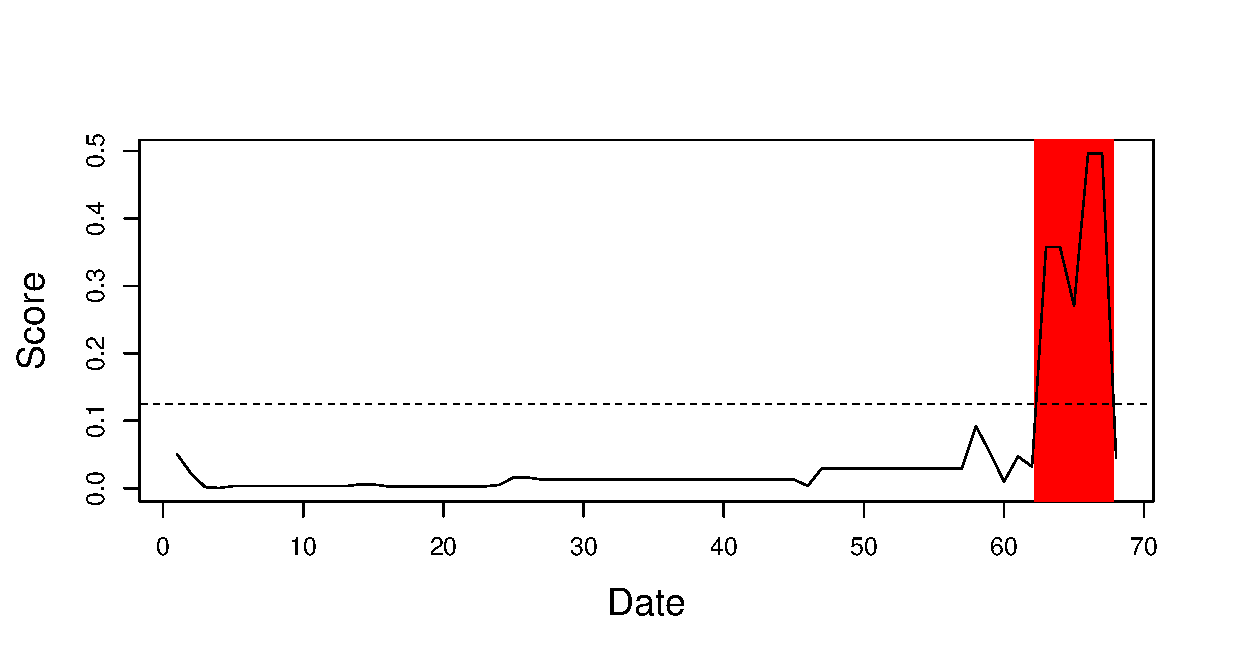
\includegraphics[width=1.0\textwidth]{longitude/figs/onePerson.eps}
%\caption{An example of diagnosing a user. On each day, a disease score (black line) is assigned to the user based on his or her Tweets. When this score exceeds a statistically derived cut off (dashed line), the user is classified as having influenza. For the case of this user, he or she has influenza for a five day period starting at day 63 (red region).}
%\label{fig:onePerson}
%\end{figure}


